%!TEX TX-program = xelatex
\documentclass[8pt]{article}
\usepackage{allan-eason}

\usetikzlibrary{positioning}
\usetikzlibrary{svg.path}

\graphicspath{ {./images/} }

\newcommand{\Date}{220507}
\newcommand{\Test}{向量}

\newcommand{\Author}{Eason S.}
\newcommand{\Title}{\textcolor{allandarkblue}{\Date}\ \textcolor{allancyan}{\Test}\ 题目选解}

\author{\Author}
\title{\Title}
\date{}

\geometry{a4paper, scale=0.8}

\lhead{\Title}

\begin{document}

	\maketitle

	\section{填空题}
		\begin{easonproblem}
			已知作用在坐标原点的三个力\(\vec{F}_1 = (3, 4), \vec{F}_2 = (2, -5), \vec{F}_3 = (3, 1)\), 则它们的合力大小为?.
			\subproblem
			\answord{\(8\).} 向量的坐标表达, 向量的和, 向量的模.
		\end{easonproblem}

		\begin{easonproblem}
			已知向量\(\vec{a} = (2, 1), A (1, 2)\), 若向量\(\ray{AB} \parallel \vec{a}\), 且\(\abs{\ray{AB}} = 2\sqrt{5}\), 则\(B\)的坐标为?.
			\subproblem
			\answord{\((5, 4) \lgor (-3, 0)\).} 向量的平行的等价命题.
		\end{easonproblem}
		
		\begin{easonbigproblem}
			已知\(P_1 (4, -3), P_2 (-2, 6)\), 若点\(P\)在线段\(P_2 P_1\)的延长线上, \(\abs{\ray{P_1 P}} = \dfrac{4}{5} \abs{\ray{P P_2}}\), 则点\(P\)的坐标是?.
			\subbigproblem
			\answord{\((28, -39)\).} 定比分点定理.
		\end{easonbigproblem}

		\begin{easonbigproblem}
			若非零向量\(\vec{a} = (x, 2x), \vec{b} = (-3x, 2)\), 且\(\ang{\vec{a}, \vec{b}} \in \left(\dfrac{\pi}{2}, \pi\right)\), 则\(x\)的取值范围是?.
			\subbigproblem
			\answord{\(\left(-\infty, -\dfrac{1}{3}\right) \cup \left(-\dfrac{1}{3}, 0\right)\cup\left(\dfrac{4}{3}, +\infty\right)\).} 向量内积取值范围与夹角的联系 (注意钝角的条件为: 内积为负且\textbf{不共线}).
		\end{easonbigproblem}

		\begin{easonproblem}
			设向量\(\vec{a}\)与\(\vec{b}\)的夹角为\(\theta\), 且\(\vec{a} = (3, 3), 2\vec{b} - \vec{a} = (-1, 1)\), 则\(\cos \theta = ?\).
			\subproblem
			\answord{\(\dfrac{3\sqrt{10}}{10}\).} 向量的坐标运算, 向量的内积.
		\end{easonproblem}

		\begin{easonproblem}
			已知\(\abs{\vec{a}} = 6, \abs{\vec{b}} = 4, \vec{a}\)与\(\vec{b}\)的夹角为\(60\degree\), 则\(\left(\vec{a} + 2\vec{b}\right)\cdot\left(\vec{a} - 3\vec{b}\right) = ?, \abs{\vec{a} + \vec{b}} = ?\).
			\subproblem
			\answord{\(-72; 2\sqrt{19}\).} 向量乘法对加法的分配律, 向量加法的平行四边形法则, 三角形中的余弦定理.
		\end{easonproblem}

		\begin{easonbigproblem}
			若\(\vec{a}=(2, 3), \vec{b}=(-4, 7), \vec{a} + \vec{c} = 0,\)则\(\vec{c}\)在\(\vec{b}\)方向上的投影为?.
			\subbigproblem
			\answord{\(-\dfrac{\sqrt{65}}{5}\).} 利用\(\displaystyle \Prj{\vec{b}}{\vec{a}} = \vec{a} \cos \ang{\vec{a}, \vec{b}} = \frac{\vec{a} \cdot \vec{b}}{\abs{\vec{b}}}\) (投影与内积的联系).
		\end{easonbigproblem}

		\begin{easonbigproblem}
			若\(\ray{OA} = (2, 3), \ray{OB} = (-4, 7), \ray{OP} = \dfrac{1}{3} \ray{OB} + \lambda \ray{OA}\). 若\(P, A, B\)三点共线, 则\(\ray{OP} = ?\).
			\subbigproblem
			\answord{\(\left(0, \dfrac{13}{3}\right)\).} 点共线与线性组合系数之间的联系.
		\end{easonbigproblem}

		\begin{easonbigproblem}
			在\(\triangle OAB\)中, \(\ray{OA} = \left(2 \cos \alpha, 2 \sin \alpha\right), \ray{OB} = \left(5 cos \beta, 5 \sin \beta\right)\), 若\(\ray{OA} \cdot \ray{OB} = 8\), 则\(S_{\triangle OAB} = ?\).
			\subbigproblem
			\answord{\(3\).} 向量的内积的定义. 本题直接使用\(\displaystyle \ray{OA} \cdot \ray{OB} = \abs{\ray{OA}} \abs{\ray{OB}} \cos \ang{\ray{OA}, \ray{OB}}\)随后解三角形较直接使用坐标内积更为简便.
		\end{easonbigproblem}

	\section{解答题}
		
		\begin{easonproblem}
			已知\(\triangle ABC\)三个顶点的直角坐标分别为\(A(3, 4), B(0, 0), C(c, 0)\),
			\begin{enumerate} [label = \calword{(\arabic*)}]
				\item 若\(\ray{AB} \cdot \ray{AC} = 0\), 求\(c\)的值.
				\item 若\(c = 5\), 求\(\sin A\)的值.
			\end{enumerate}
			\subproblem
			\answord{\(\dfrac{25}{3}; \dfrac{2\sqrt{5}}{5}\).} 向量的坐标内积, 过程略.
		\end{easonproblem}

		\begin{easonproblem}
			已知\(\abs{\vec{a}} = \abs{\vec{b}} = 1\), \(\vec{a}\)与\(\vec{b}\)的夹角为\(\dfrac{\pi}{3}\), \(\vec{x} = 2\vec{a} - \vec{b}, \vec{y} = 3\vec{b} - \vec{a}\), 求\(\vec{x}\)与\(\vec{y}\)的夹角.
			\subproblem
			\answord{\(\arccos\left(-\dfrac{\sqrt{21}}{14}\right)\).} 向量的内积.
			\begin{align*}
				\cos \ang{\vec{x}, \vec{y}} &= \frac{\vec{x} \cdot \vec{y}}{\abs{\vec{x}} \abs{\vec{y}}}\\
											&= \frac{- 2\vec{a}^2 + 7\vec{a} \cdot \vec{b} - 3\vec{b}^2}{\sqrt{\left(2\vec{a} - \vec{b}\right)^2 \left(3\vec{b} - \vec{a}\right)^2}}\\
											&= \frac{-2\abs{\vec{a}}^2 + 5\abs{\vec{a}} \abs{\vec{b}} \cos \frac{\pi}{3} - 3\abs{\vec{b}}^2}{\sqrt{\left(4\vec{a}^2 + \vec{b}^2 - 4\vec{a} \cdot \vec{b}\right)\left(9\vec{b}^2 + \vec{a}^2 - 6 \vec{a} \cdot \vec{b}\right)}}\\
											&= \frac{-2 + \frac{7}{2} - 3}{\sqrt{3 \times 7}}\\
											&= - \frac{\sqrt{21}}{14}.
			\end{align*}
		\end{easonproblem}

		\begin{easonproblem}
			如图, 在梯形\(ABCD\)中\(\ray{AB}=\vec{a}, \ray{BC}=\vec{b}, \ray{CD}=\dfrac{1}{2}\vec{a}, G\)为对角线\(AC, BD\)的交点, \(E, F\)分别是腰\(AD, BC\)的中点, 求向量\(\ray{EF}\)和\(\ray{AG}\).
			\[
				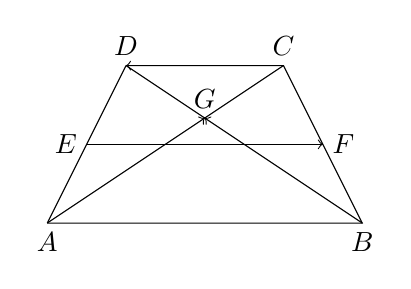
\begin{tikzpicture}
					\draw[black, ->] (0, 0)--(4, 0)--(3, 2)--(1, 2) node at (0, 0) [anchor = north] {\(A\)} node at (4, 0) [anchor = north] {\(B\)} node at (3, 2) [anchor = south] {\(C\)} node at (1, 2) [anchor = south] {\(D\)};
					\draw[black] (1, 2)--(0, 0);
					\draw[black, ->] (0.5, 1)--(3.5, 1) node at (0.5, 1) [anchor = east] {\(E\)} node at (3.5, 1) [anchor = west] {\(F\)};
					\draw[black, ->] (0, 0)--(2, {4/3});
					\draw[black, ->] (4, 0)--(2, {4/3});
					\draw[black] (1, 2)--(2, {4/3})--(3, 2) node at (2, {4/3}) [anchor = south] {\(G\)};
				\end{tikzpicture}
			\]
			\subproblem
			\answord{\(\ray{EF} = \dfrac{3}{4}\vec{a}, \ray{AG} = \dfrac{2}{3}\vec{a} + \dfrac{2}{3}\vec{b}\).} 向量的线性组合.
		\end{easonproblem}

		\begin{easonbigproblem}
			已知向量\(\vec{a} = (1, 2), \vec{b} = (-3, 2)\), 向量\(\vec{x} = k\vec{a} + \vec{b}, \vec{y} = \vec{a} - 3\vec{b}\).
			\begin{enumerate} [label = \calword{(\arabic*)}]
				\item 当\(k\)为何值时, 向量\(\vec{x} \perp \vec{y}\).
				\item 若向量\(\vec{x}\)与\(\vec{y}\)的夹角为钝角, 求实数\(k\)的取值范围.
			\end{enumerate}
			\subbigproblem
			\answord{\(k=19; k\in \left(-\infty, -\dfrac{1}{3}\right)\cup\left(-\dfrac{1}{3}, 19\right)\).} 向量内积取值范围与夹角的联系.
		\end{easonbigproblem}

		\begin{easonbigproblem}
			已知向量\(\vec{a} = (\sin x, \cos x), \vec{b} = (\sin x, \sin x), \vec{c} = (-1, 0)\).
			\begin{enumerate} [label = \calword{(\arabic*)}]
				\item 若\(x = \dfrac{\pi}{3}\), 求向量\(\vec{a}, \vec{c}\)的夹角\(\theta\).
				\item 若\(x \in \left[-\dfrac{3\pi}{8}, \dfrac{\pi}{4}\right]\), 函数\(f(x) = \lambda \vec{a} \cdot \vec{b}\)的最大值为\(\dfrac{1}{2}\), 求实数\(\lambda\)的值.
			\end{enumerate}
			\subbigproblem
			\answord{\(\theta = \dfrac{5\pi}{6}; \lambda = \dfrac{1}{2} \lgor \lambda = -\sqrt{2}-1\).} 向量的内积的定义; 三角函数的极值.
			\begin{enumerate} [label = \calword{(\arabic*)}]
				\item \(\vec{a} = \left(\sin \dfrac{\pi}{3}, \cos \dfrac{\pi}{3}\right) = \left(\dfrac{\sqrt{3}}{2}, \dfrac{1}{2}\right) = \left(\cos \dfrac{\pi}{6}, \sin \dfrac{\pi}{6}\right), \vec{c} = (-1, 0) = \left(\cos \pi, \sin \pi\right) \Rightarrow \theta = \pi - \dfrac{\pi}{6} = \dfrac{5\pi}{6}.\)
				\item \(f(x) = \lambda \left(\sin^2 x + \sin x \cos x\right) = \lambda \left[\dfrac{\sqrt{2}}{2} \sin \left(2x - \dfrac{\pi}{4}\right) + \dfrac{1}{2}\right]\).
				
				\(x \in \left[-\dfrac{3\pi}{8}, \dfrac{\pi}{4}\right] \Rightarrow 2x - \dfrac{\pi}{4} \in \left[-\pi, \dfrac{\pi}{4}\right] \Rightarrow \sin \left(2x - \dfrac{\pi}{4}\right) \in \left[-1, \dfrac{\sqrt{2}}{2}\right].\)
				
				考虑\(\lambda > 0\), 有\(x = \dfrac{\pi}{4}\)时\(f_{\max}(x)=\lambda=\dfrac{1}{2}\), 即\(\lambda = \dfrac{1}{2}\);
				
				考虑\(\lambda < 0\), 有\(x = -\dfrac{\pi}{8}\)时\(f_{\max}(x) = \dfrac{1 - \sqrt{2}}{2} \lambda = \dfrac{1}{2}\), 即\(\lambda = -\sqrt{2} - 1\).
			\end{enumerate}
		\end{easonbigproblem}

	\section{附加题}

		\begin{easonbigproblem}
			已知向量\(\vec{m} = (\sqrt{3}, 1)\), 向量\(\vec{n}\)是与向量\(\vec{m}\)夹角为\(\dfrac{\pi}{3}\)的单位向量.
			\begin{enumerate} [label = \calword{(\arabic*)}]
				\item 求向量\(\vec{n}\).
				\item 若向量\(\vec{n}\)与向量\(\vec{q} = \left(-\sqrt{3}, 1\right)\)平行, 与向量\(\vec{p} = \left(\sqrt{3} x^2, x - y^2\right)\)垂直, 求\(t = y^2 + 5x + 4\)的最大值.
			\end{enumerate}
			\subbigproblem
			\answord{\(\vec{n} = (0, 1) \lgor \left(\dfrac{\sqrt{3}}{2}, -\dfrac{1}{2}\right); t_{\max} = \dfrac{17}{3}\).} 向量内积取值范围与夹角的联系 / 变换矩阵; 二次函数最值.
			\begin{enumerate} [label = \calword{(\arabic*)}]
				\item	\athword{法一: } \(\vec{m} = \left(2 \cos \dfrac{\pi}{6}, 2 \sin \dfrac{\pi}{6}\right),\) 又\(\ang{\vec{m}, \vec{n}}=\dfrac{\pi}{3}\), 有\(\vec{n} = \left(\cos \left(\dfrac{\pi}{6} + \dfrac{\pi}{3}\right), \sin \left(\dfrac{\pi}{6} + \dfrac{\pi}{3}\right)\right) = (0, 1)\)或\(\vec{n} = \left(\cos \left(\dfrac{\pi}{6} - \dfrac{\pi}{3}\right), \sin \left(\dfrac{\pi}{6} - \dfrac{\pi}{3}\right)\right) = \left(\dfrac{\sqrt{3}}{2}, -\dfrac{1}{2}\right)\).
    
						\athword{法二: } 
						\[
							k \vect{n} = \vect{m} \left[
								\begin{array}{cc}
									\cos \varphi & -\sin \varphi\\
									\sin \varphi & \cos \varphi
								\end{array}
							\right] (\text{顺时针旋转}\varphi),
						\]
						其中\(\varphi = \pm \dfrac{\pi}{3}, k \in \RR\), 于是有
						\begin{align*}
							k \vect{n} &= \vect{m} \left[
								\begin{array}{cc}
									\cos \varphi & -\sin \varphi\\
									\sin \varphi & \cos \varphi
								\end{array}
							\right]\\
									 &= 
									 \left[\sqrt{3}, 1\right]
									 \left[
										\begin{array}{cc}
											\cos \frac{\pi}{3} & - \sin \frac{\pi}{3}\\
											\sin \frac{\pi}{3} & \cos \frac{\pi}{3}
										\end{array}
									\right]\\
									 &= 
									 \left[\sqrt{3}, 1\right]
									 \left[
										\begin{array}{cc}
											\frac{1}{2} & - \frac{\sqrt{3}}{2}\\
											\frac{\sqrt{3}}{2} & \frac{1}{2}
										\end{array}
									\right]\\
									 &= \left[\sqrt{3}, -1\right], k = 2, \vect{n} = \left[\frac{\sqrt{3}}{2}, -\dfrac{1}{2}\right].
						\end{align*}
						\[\lgor\]
						\begin{align*}
							k \vect{n} &= \vect{m} \left[
								\begin{array}{cc}
									\cos \varphi & -\sin \varphi\\
									\sin \varphi & \cos \varphi
								\end{array}
							\right]\\
									 &= 
									 \left[\sqrt{3}, 1\right]
									 \left[
										\begin{array}{cc}
											\cos - \frac{\pi}{3} & - \sin - \frac{\pi}{3}\\
											\sin - \frac{\pi}{3} & \cos - \frac{\pi}{3}
										\end{array}
									\right]\\
									 &= 
									 \left[\sqrt{3}, 1\right]
									 \left[
										\begin{array}{cc}
											\frac{1}{2} & \frac{\sqrt{3}}{2}\\
											- \frac{\sqrt{3}}{2} & \frac{1}{2}
										\end{array}
									\right]\\
									 &= \left[0, 2\right], k = 2, \vect{n} = \left[0, 1\right].
						\end{align*}
				\item \[\vec{n} \parallel \left(-\sqrt{3}, 1\right) \Rightarrow \vec{n} = \left(\dfrac{\sqrt{3}}{2}, -\dfrac{1}{2}\right),\]
				\begin{align*}
					\vec{n} \perp \left(\sqrt{3}x^2, x-y^2\right) &\Rightarrow \dfrac{3}{2} x^2 - \dfrac{x}{2} + \dfrac{y^2}{2} = 0\\
					&\Rightarrow y^2 = x - 3x^2 \geq 0\\
					&\Rightarrow x \in \left[0, \dfrac{1}{3}\right]\\
					&\Rightarrow t = -3x^2 + 6x + 4 = -3(x-1)^2 + 7.
				\end{align*}

				\(t_{\max} = \dfrac{17}{3} \Iff (x, y) = \left(\dfrac{1}{3}, 0\right)\).

			\end{enumerate}
		\end{easonbigproblem}
		
\end{document}